\newpage

\paragraph{\LARGE Aufgabe 5 - Simulation der Scheduling-Algoritmen}

\section{Aufgabe 5.1}
	\subsection{Aufgabenstellung}
		\begin{quote}
			F\"uhren Sie eine Handsimulation der Scheduling-Algoritmen auf dem beiligenden \"Ubungsblatt mit den angegebenen Werten durch.\\
		\end{quote}
	\subsection{Vorbereitung}
		\begin{quote}
			Vorlesung drei lesen.\\
		\end{quote}
	\subsection{Durchführung}
		\begin{quote}
			Aufgaben auf Papier l\"osen und dann einscannen.\\
		\end{quote}
	\subsection{Fazit}
		\begin{quote}
			First-Come-First-Served\\
			Die Reihenfolge ist die Eingangsreihenfolge A, B, C, D, E:\\
			\begin{figure}[h]
				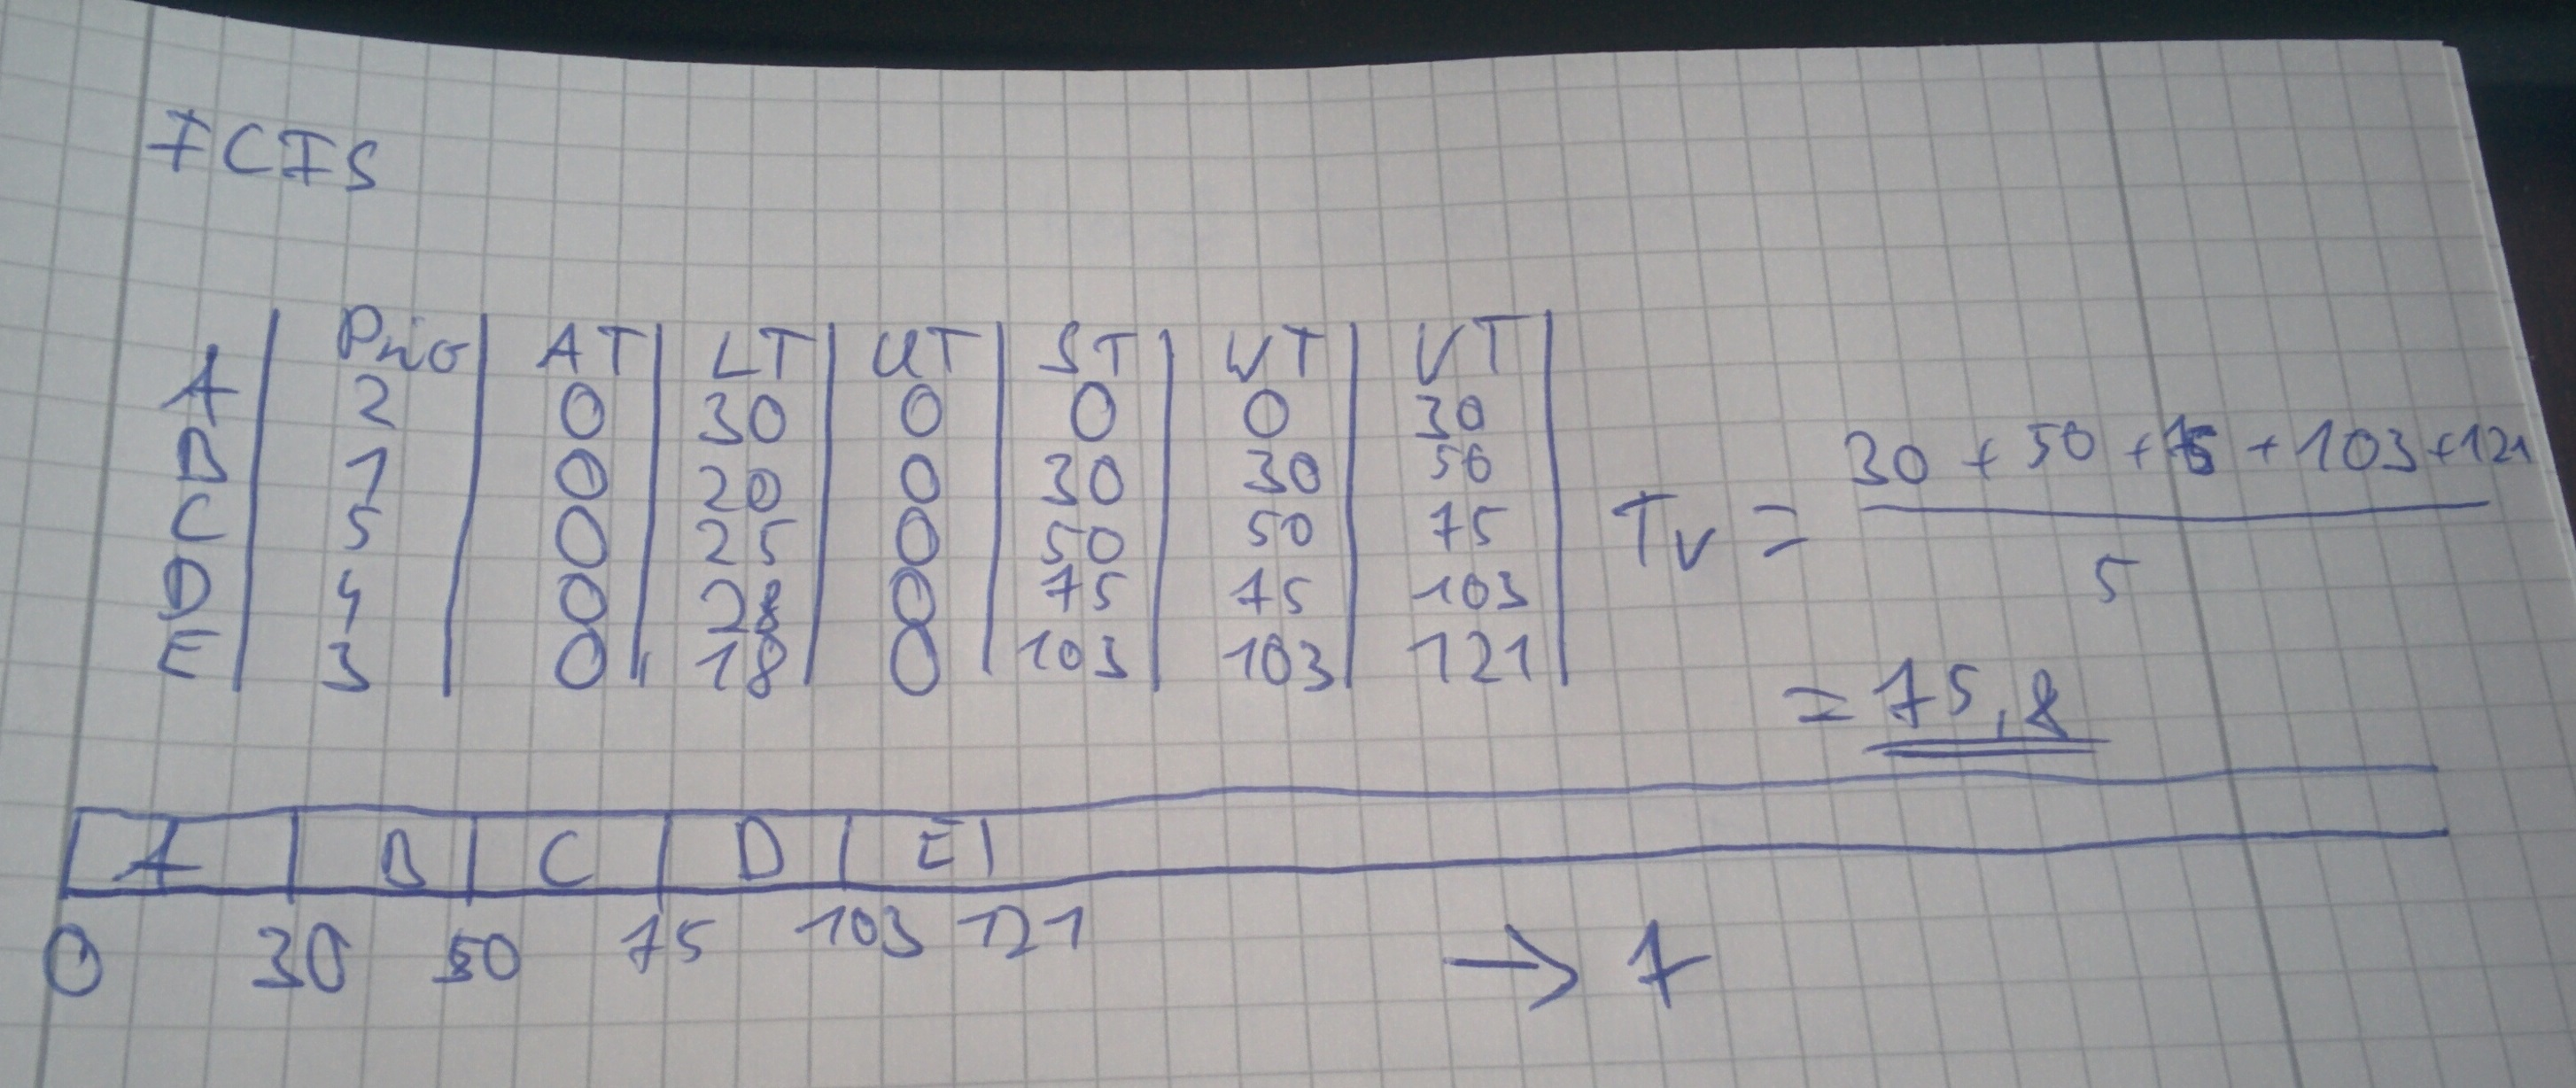
\includegraphics[width=0.7\linewidth]{content/FCFS}
				\caption{}
				\label{fig:FCFS}
			\end{figure}
			\newpage
			Shortest Job First\\ 
			Die Reihenfolge ist E, B, C, D, A:\\
			\begin{figure}[h]
				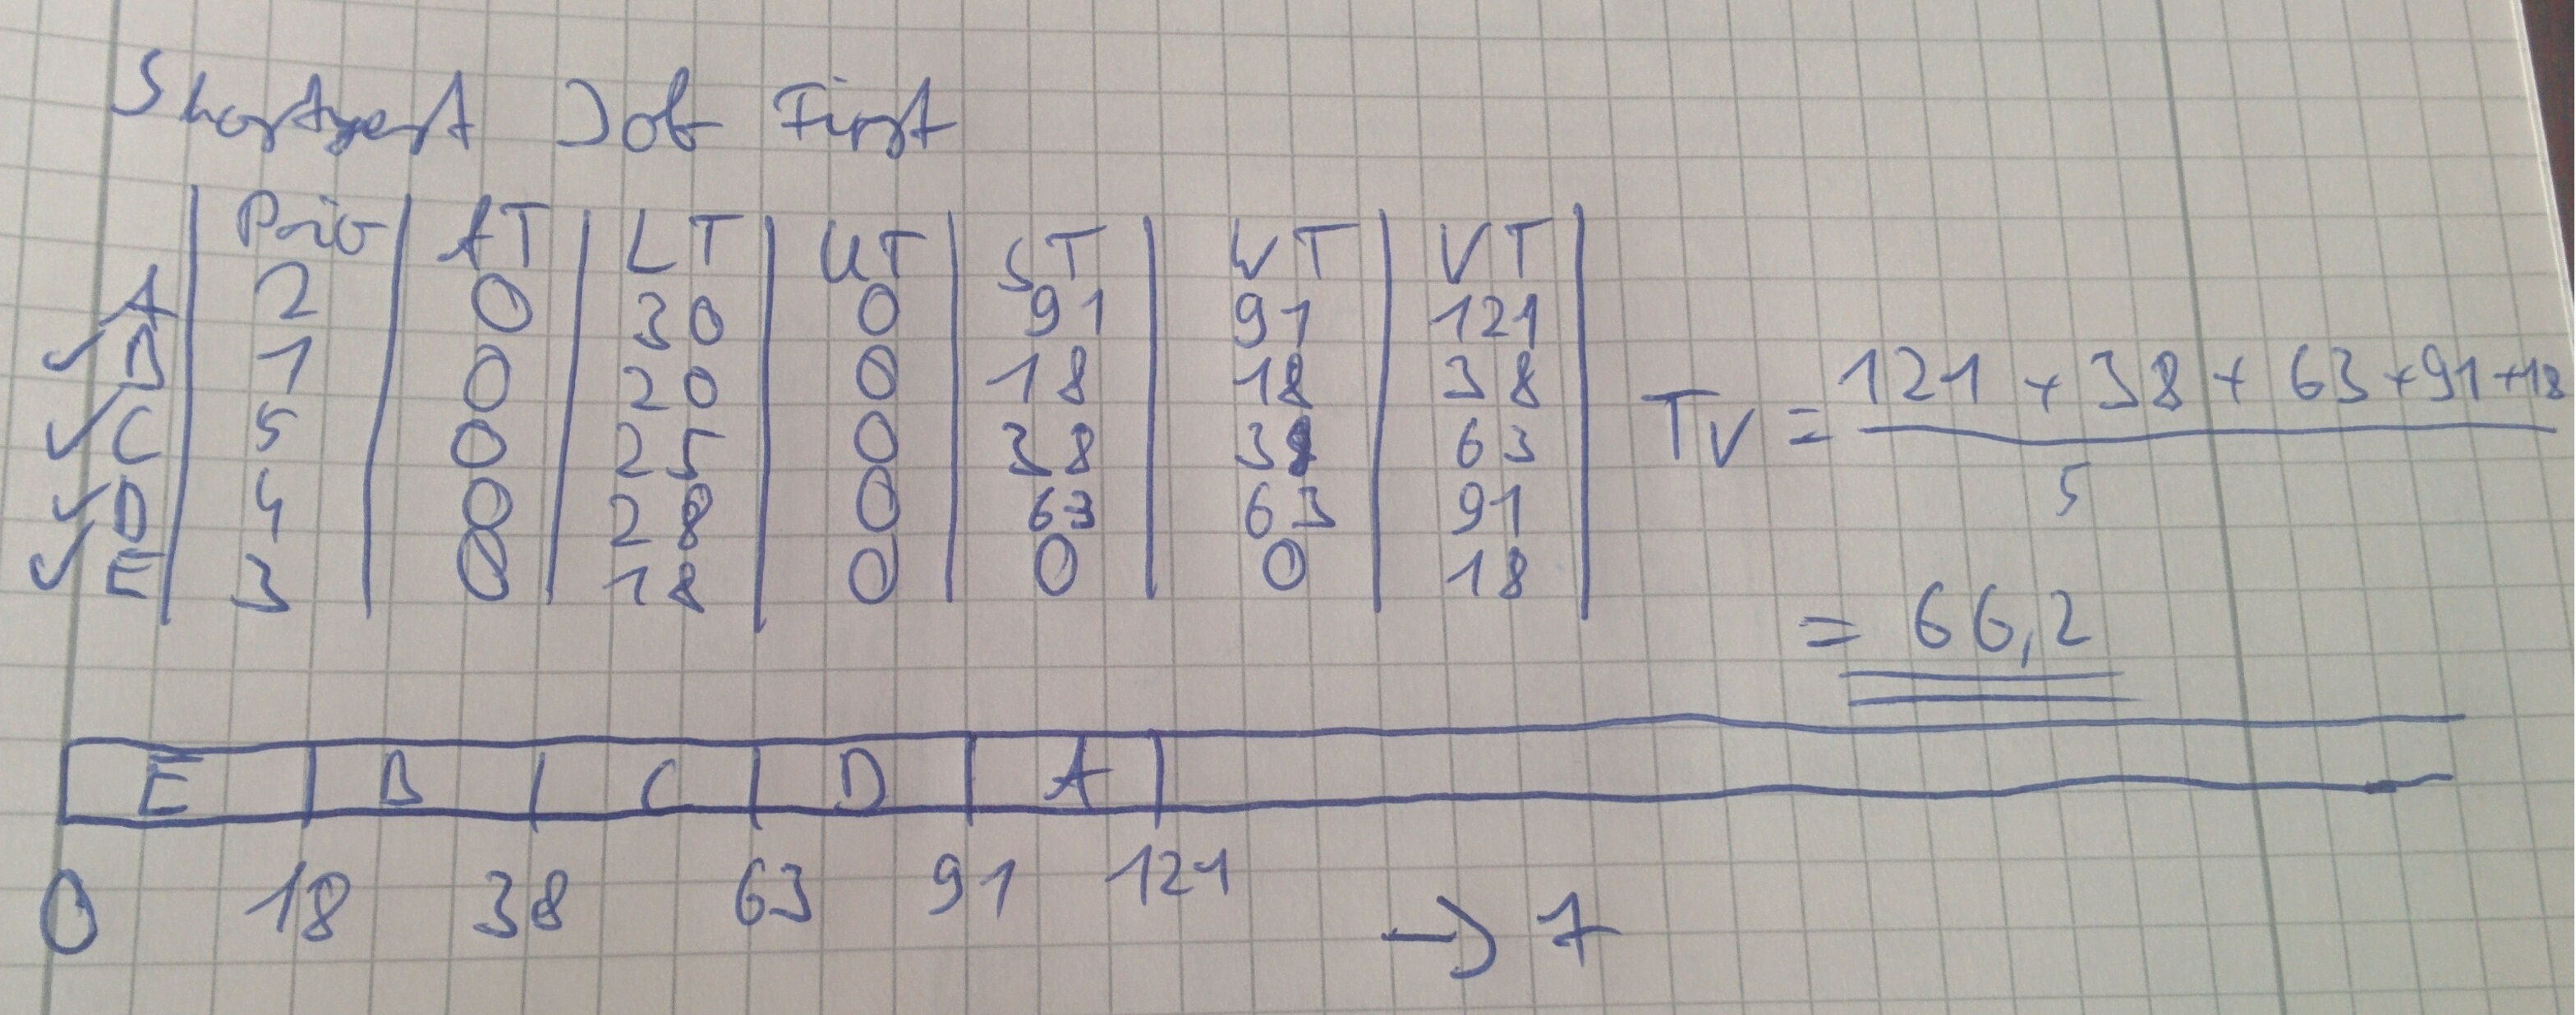
\includegraphics[width=0.7\linewidth]{content/SJF}
				\caption{}
				\label{fig:SJF}
			\end{figure}
			\newpage
			Priorisiertes Scheduling\\
			Die Reihenfolge ist C, D, E, A, B:\\
			\begin{figure}[h]
				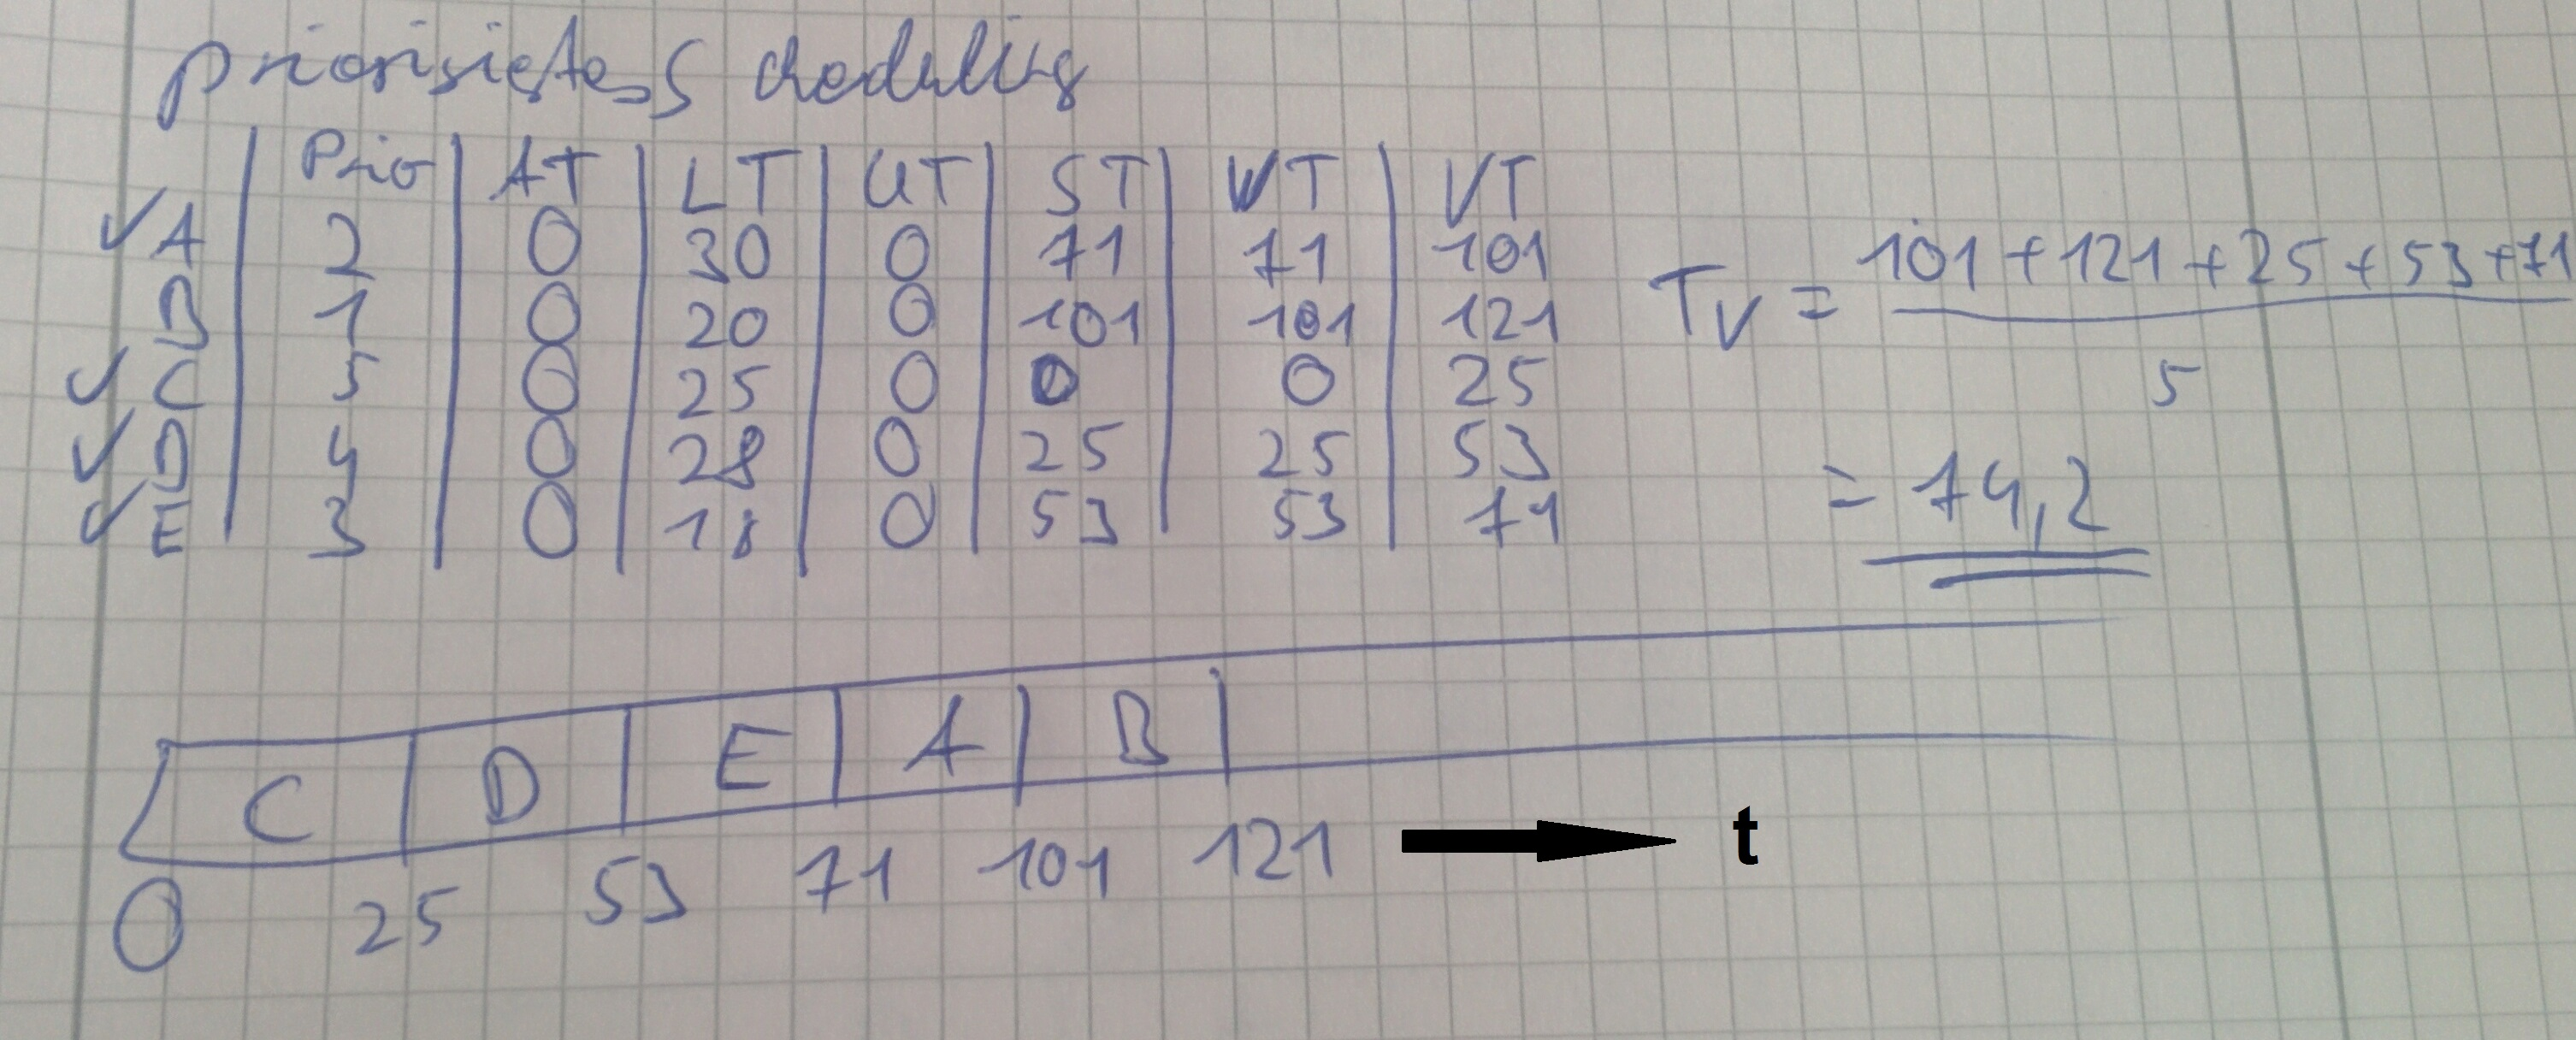
\includegraphics[width=0.7\linewidth]{content/PS}
				\caption{}
				\label{fig:PS}
			\end{figure}
			\newpage
			Round Robin mit konstanter Zeitscheibe unabh\"anig von der Priorit\"at\\
			\begin{figure}[h]
				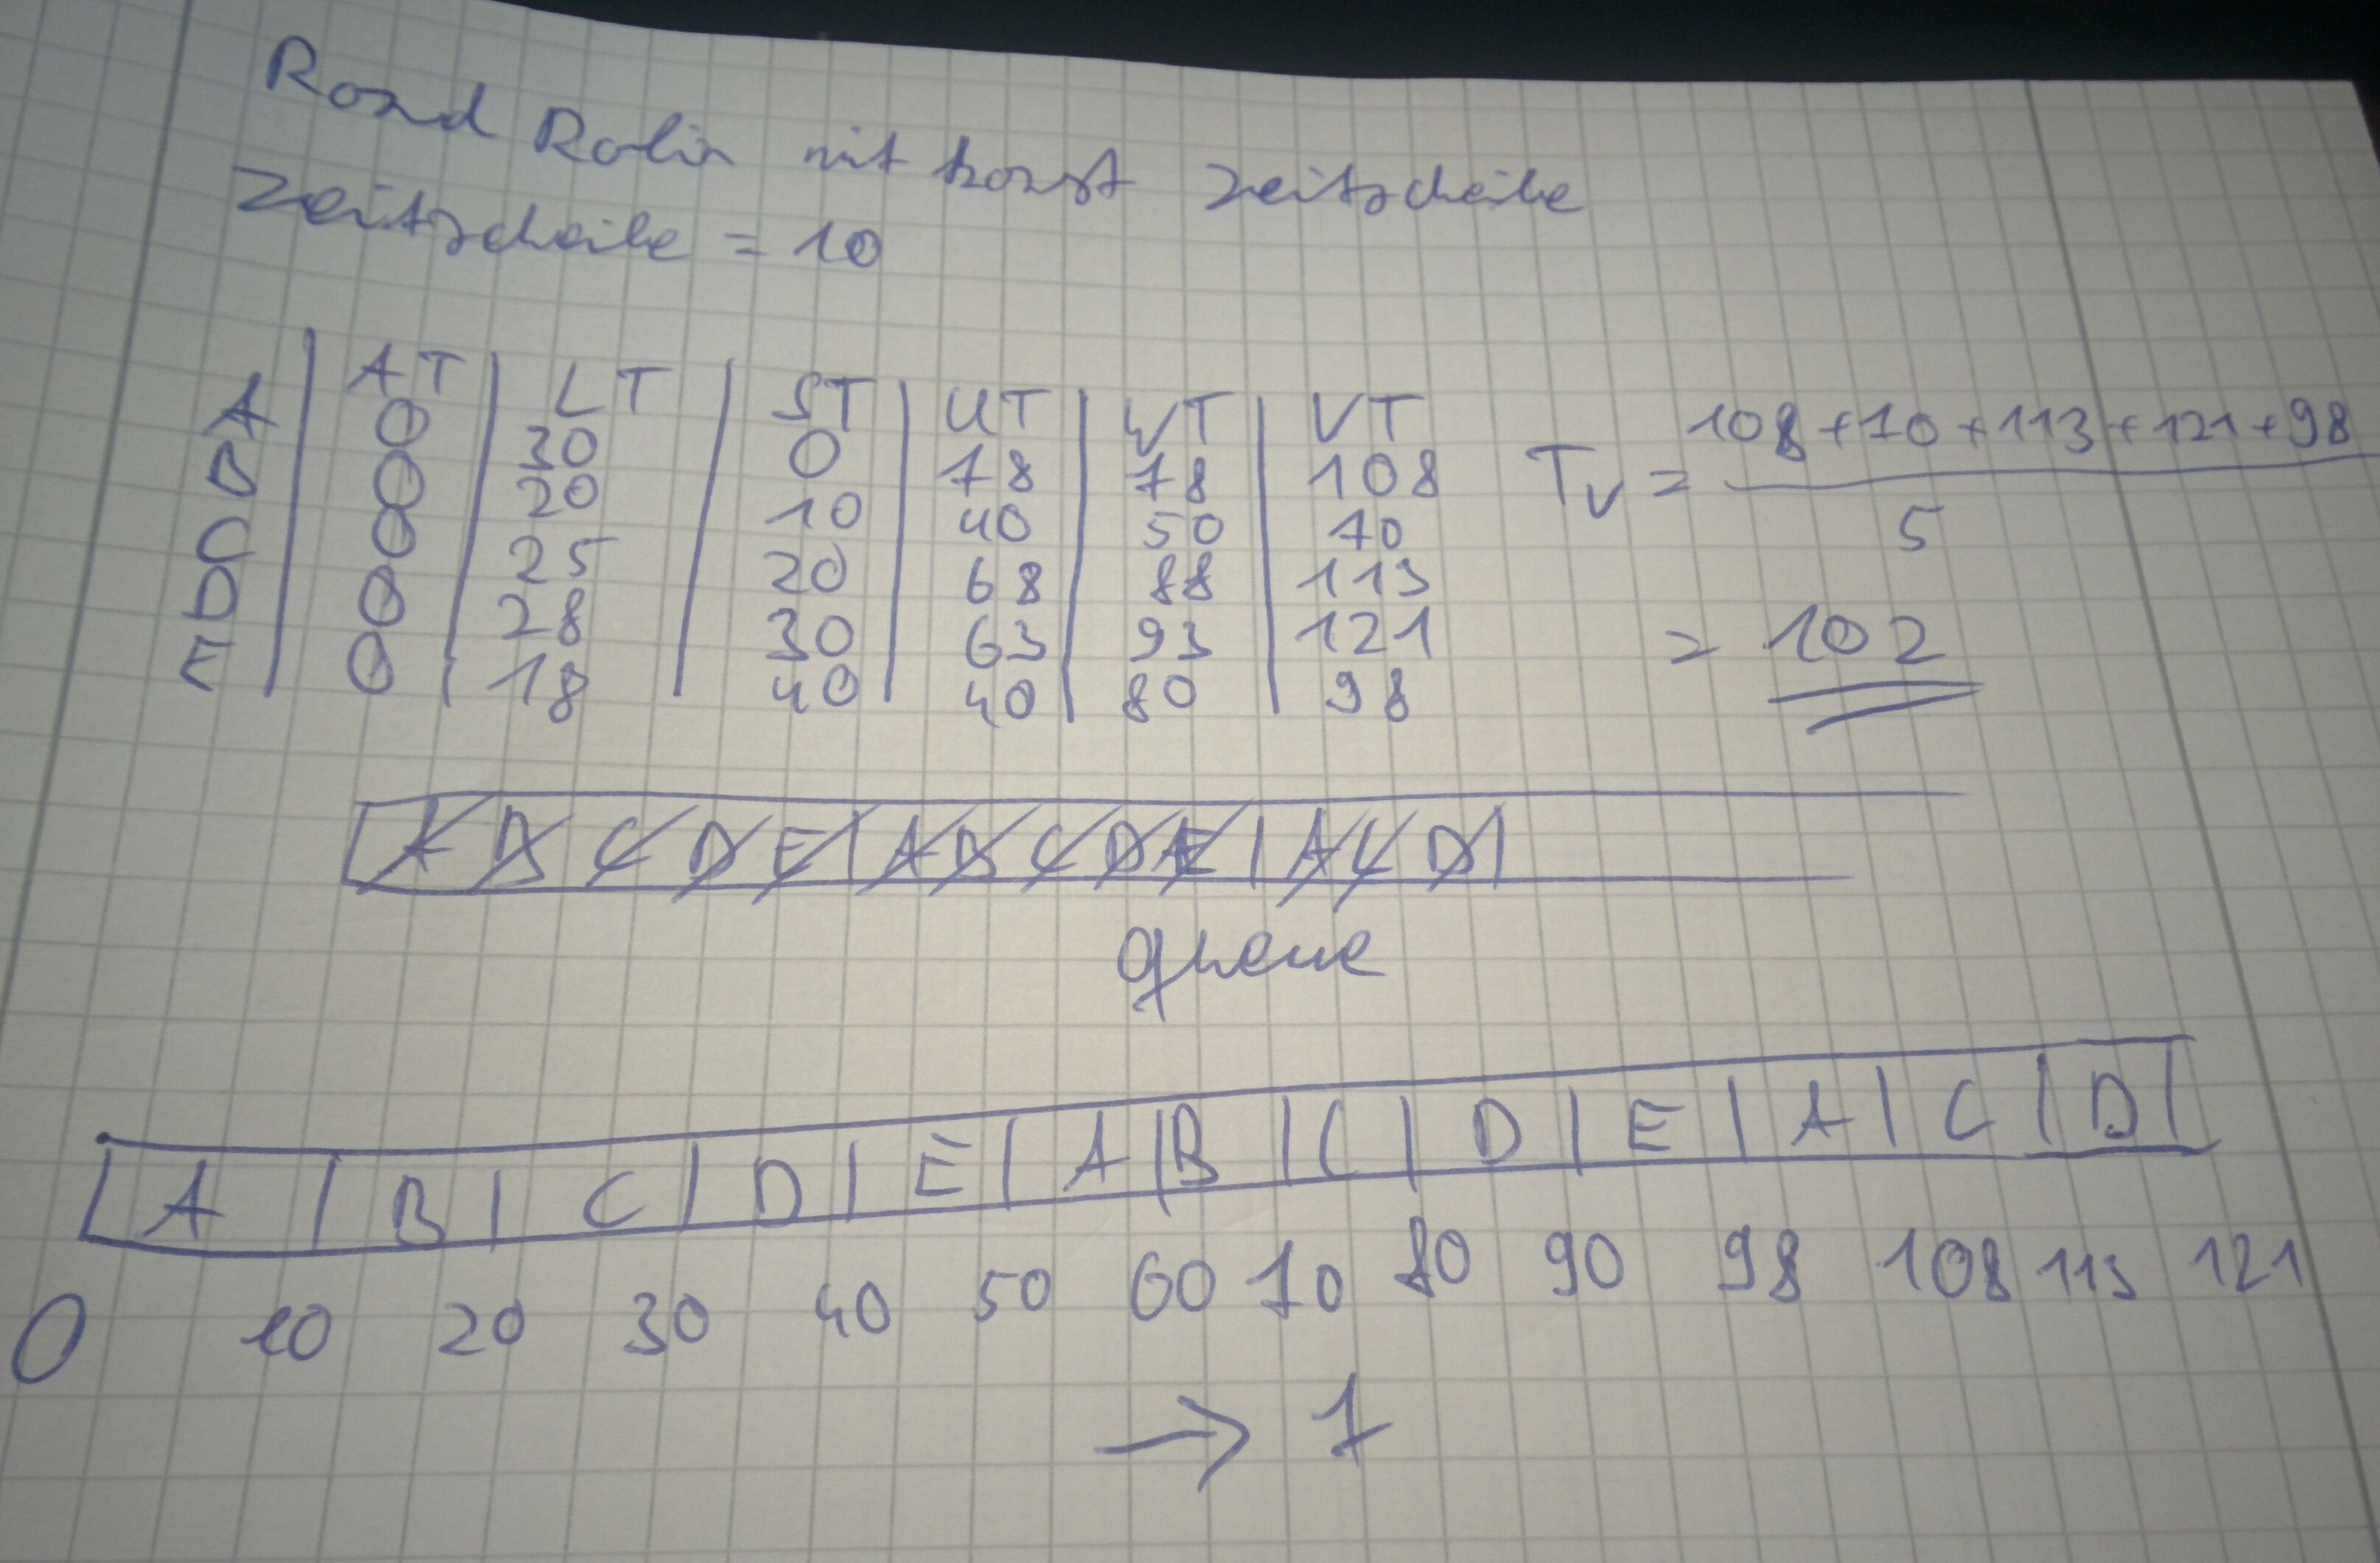
\includegraphics[width=0.7\linewidth]{content/RR}
				\caption{}
				\label{fig:RR}
			\end{figure}
			\newpage
			Round Robin mit Zeitscheibendauer proportional zur  Priorit\"at\\
			\begin{figure}[h]
				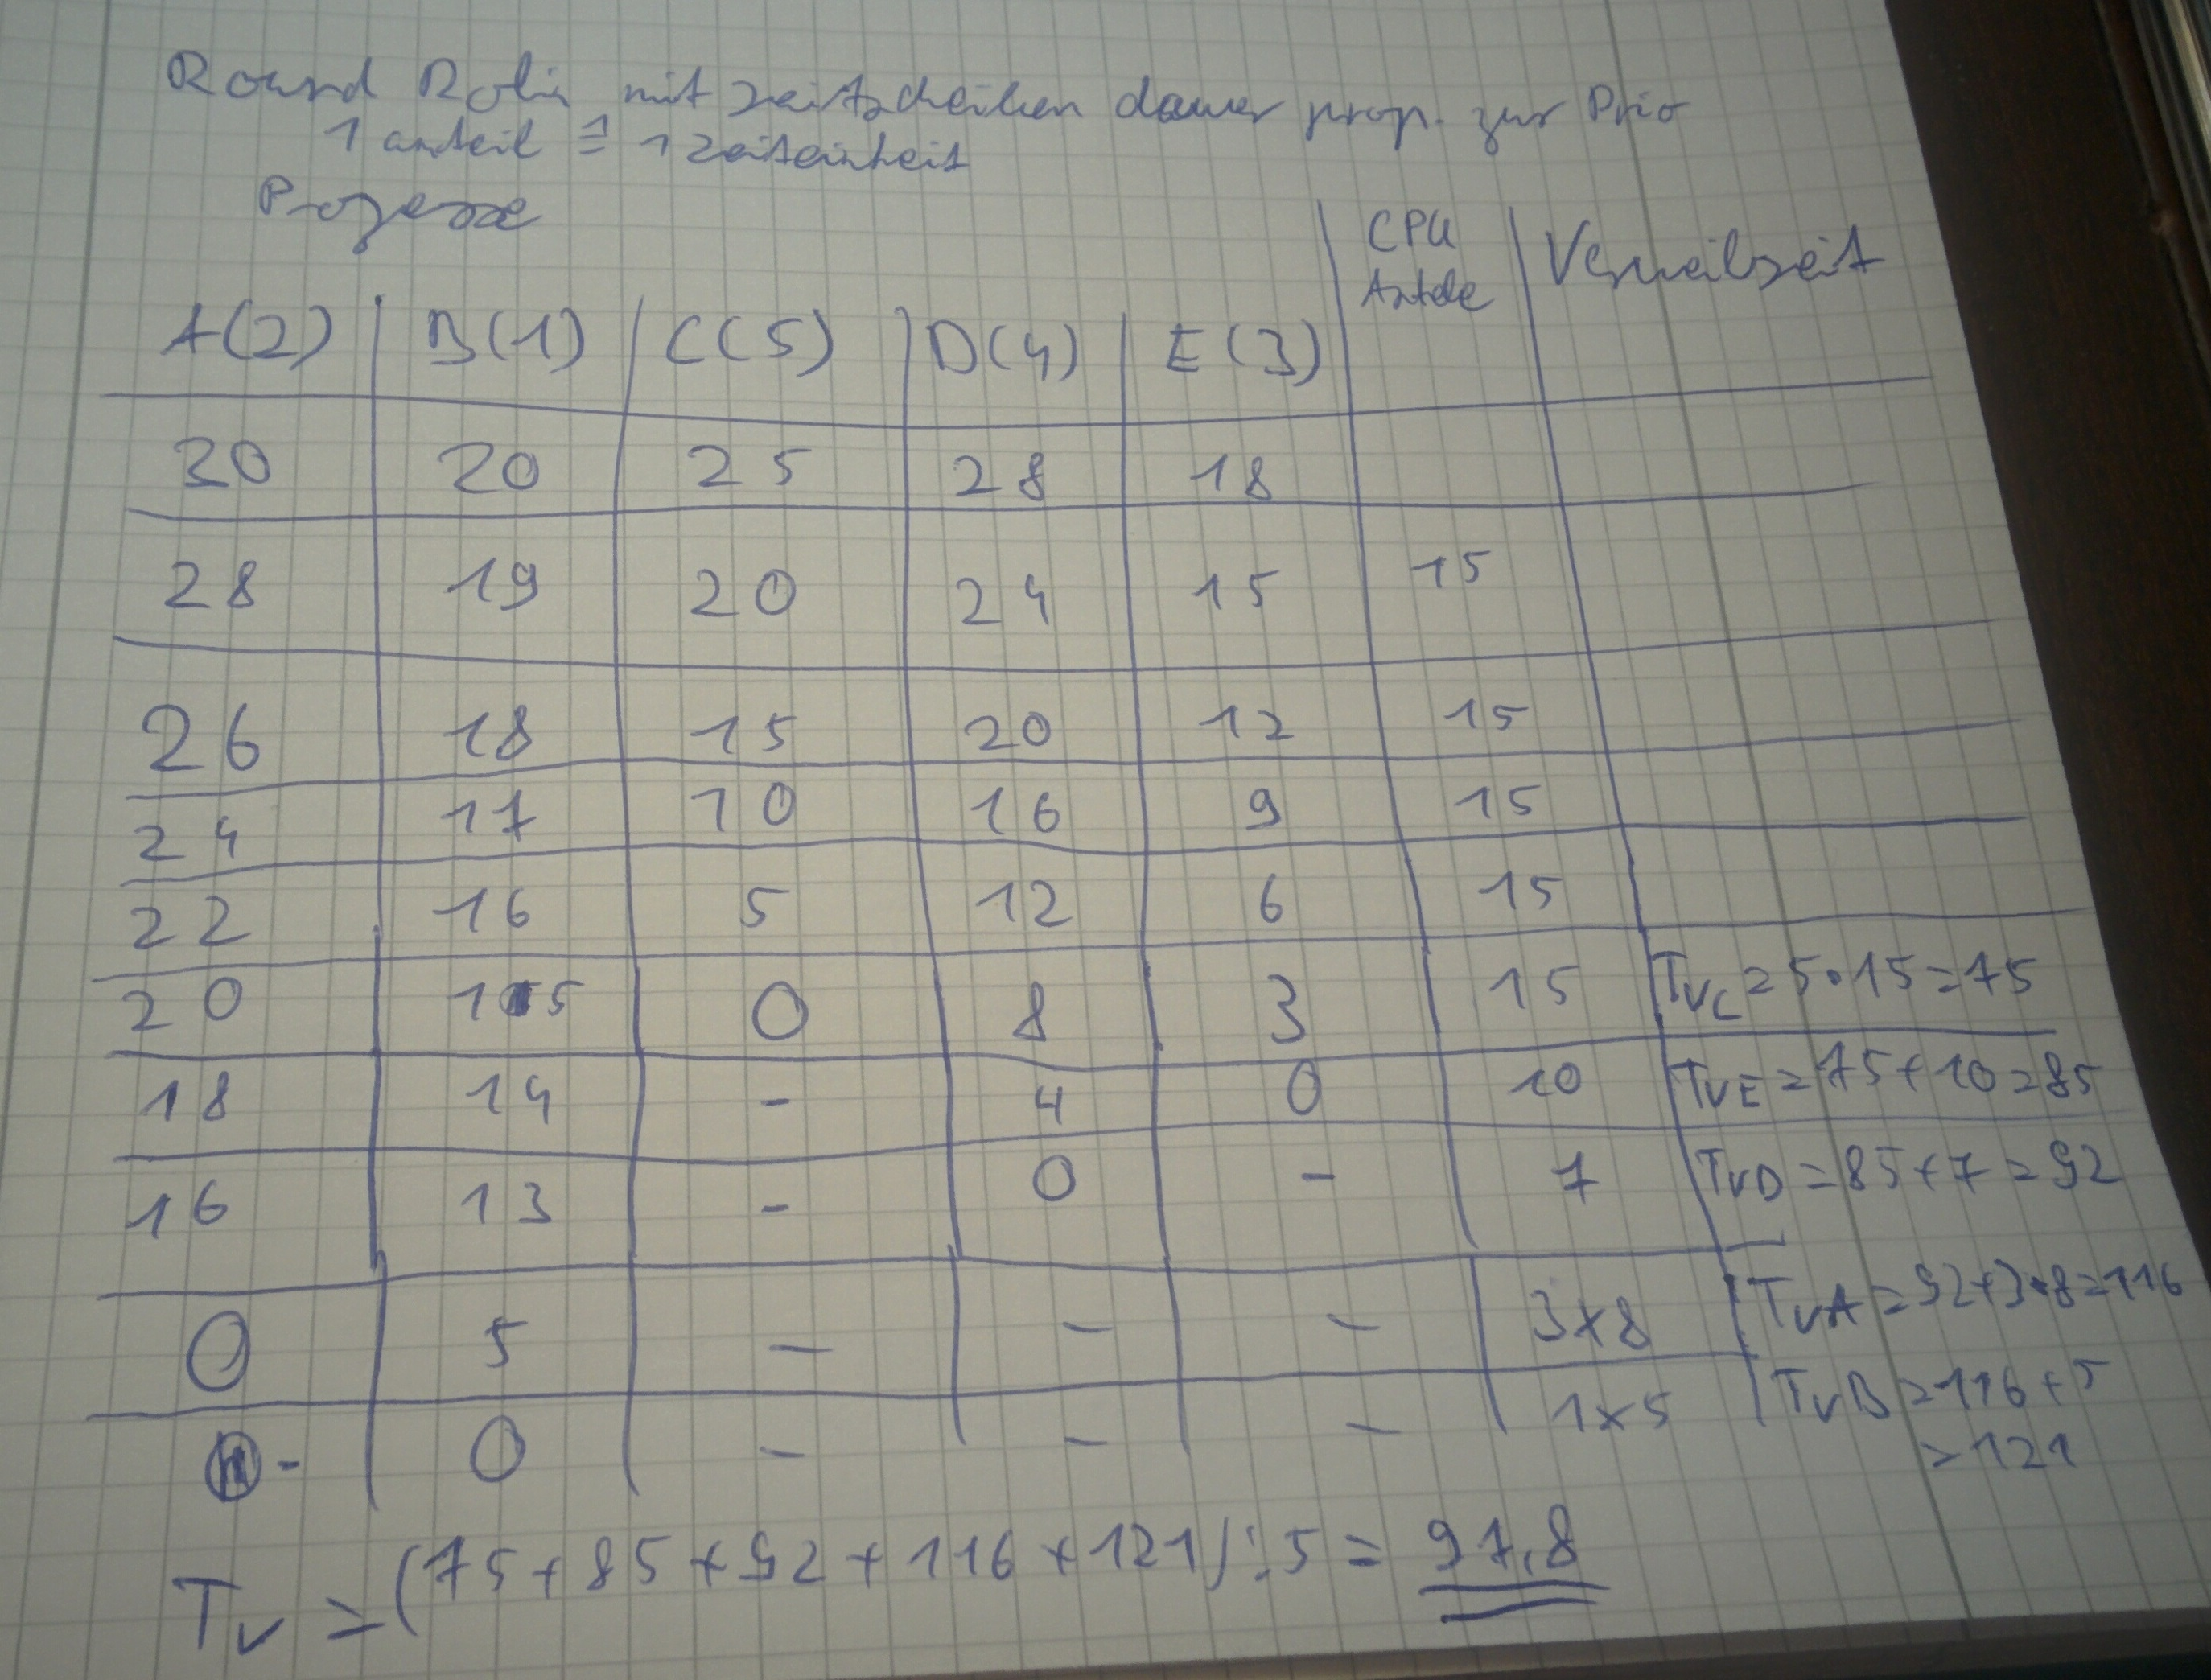
\includegraphics[width=0.7\linewidth]{content/PPRR}
				\caption{}
				\label{fig:PPRR}
			\end{figure}

		\end{quote}
\newpage
\section{Aufgabe 5.2}
	\subsection{Aufgabenstellung}
		\begin{quote}
			Implementieren Sie folgende in der Vorlesung behandelte Scheduling-Algoritmen:\\
			\begin{itemize}
				\item First Come First Served\\
				\item Shortest Job First\\
				\item priorit\"atsgesteuertes Scheduling\\
				\item Round Robin mit konstanter Zeitscheibe unabh\"anig von der Priorit\"at\\
				\item Round Robin mit Zeitscheibendauer proportional zur  Priorit\"at\\
			\end{itemize}
			Ihr Programm soll die Algorithmen vollst\"andig simulieren. Außerdem soll die mittlere Verweilzeit bestimmt werden. Verwenden Sie zur Simulation der Abl\"aufe eine Liste von	Jobs. Jeder Job speichert seinen Namen, seine Abarbeitungszeit und seine Priorit\"at. Sie k\"onnen zur vereinfachten Umsetzung die beiliegende Liste verwenden. Die Ausgaben sollen folgendermaßen aussehen und bei jedem Zeitschritt ausgegeben werden:\\ \\
			\textbf{Beispielausgabe zu First Come First Served:}\\
			a wurde abgearbeitet (Aktuelle Zeit: xx).\\
			b wurde abgearbeitet (Aktuelle Zeit: xx).\\
			c wurde abgearbeitet (Aktuelle Zeit: xx).\\
			d wurde abgearbeitet (Aktuelle Zeit: xx).\\
			e wurde abgearbeitet (Aktuelle Zeit: xx).\\
			Mittlere Verweilzeit: xx.xx s\\ \\
			\textbf{Beispielausgabe zu Round Robin:}\\
			Es wird an den Jobs zu folgenden Anteilen gearbeitet:\\
			Es wurde 1s an a gearbeitet.\\
			Es wurde 1s an b gearbeitet.\\
			Es wurde 1s an c gearbeitet.\\
			Es wurde 1s an d gearbeitet.\\
			Es wurde 1s an e gearbeitet.\\ \\
			Es wird an den Jobs zu folgenden Anteilen gearbeitet:\\
			...\\ \\
			Testen Sie alle f\"unf Algorithmen mit einer Reihe von Jobs verschiedener Gr\"oße und vergleichen Sie die Ergebnisse. Testen Sie die Algorithmen ebenfalls f\"ur die im ersten Aufgabenteil vorgegebenen Jobs. Anhand der Ergebnisse k\"onnen Sie \"uberpr\"ufen, ob Sie die Algorithmen korrekt implementiert haben.\\
		\end{quote}
	\subsection{Vorbereitung}
		\begin{quote}
			C-Projekt von p04 in Master Mergen.\\
			C-Projekt aufr\"aumen.\\
			Makefile \"andern.\\
			Zu branch p05 wechseln.\\
		\end{quote}
	\subsection{Durchführung}
		\begin{quote}
			Code schreiben und dann testen bzw debuggen.
		\end{quote}
	\subsection{Fazit}
		\begin{quote}
			\lstinputlisting[language=C, firstline=13, lastline=23]{../src/myScheduler.c}
			Hier wird der Job und die JobList definiert.\\
			
			\lstinputlisting[language=C, firstline=25, lastline=35]{../src/myScheduler.c}
			Die Methode vergleicht die Listen Element anhand der Id.\\
			
			\lstinputlisting[language=C, firstline=37, lastline=47]{../src/myScheduler.c}
			Die Methode vergleicht die Listen Element anhand der Laufzeit.\\
			
			\lstinputlisting[language=C, firstline=49, lastline=59]{../src/myScheduler.c}
			Die Methode vergleicht die Listen Element anhand der Priorit\"at.\\
			
			\lstinputlisting[language=C, firstline=63, lastline=101]{../src/myScheduler.c}
			Mit der Methode wird eine Beispielliste erstellt.\\
			First Come First Served\\
			\lstinputlisting[language=C, firstline=105, lastline=117]{../src/myScheduler.c}
			Die Liste wird Element f\"ur Element durch gegangen. Dabei werden die Zeiten aufsummiert(Gesamtzeit und Verweiltezeitgesammt) und die Einzelnen Ausgaben get\"atigt. Am ende wird die Mittlere Verweiltezeit berechnet.\\
			Shortest Job First\\
			\lstinputlisting[language=C, firstline=119, lastline=131]{../src/myScheduler.c}
			Wie bei FCFS nur das die Liste nach Laufzeiten sortiert wird.
			priorit\"atsgesteuertes Scheduling\\
			\lstinputlisting[language=C, firstline=133, lastline=145]{../src/myScheduler.c}
			Wie bei FCFS nur das die Liste nach Priorit\"aten sortiert wird.\\
			Raund Robin\\
			\lstinputlisting[language=C, firstline=147, lastline=175]{../src/myScheduler.c}
			Zuerst wird nach ID sortiert. Dann werden so oft Zeitscheiben abgezogen bis alle Laufzeiten < 1 sind. Die laufzeiten die < 1 sind werden \"bersprungen.\\
			Round Robin mit Priorit\"aten\\
			
			\lstinputlisting[language=C, firstline=177, lastline=204]{../src/myScheduler.c}
			Wie Round Robin nur die Zeinscheiben sind gleich der Priorit\"at.\\
		\end{quote}